\documentclass[]{article}
\usepackage{lmodern}
\usepackage{amssymb,amsmath}
\usepackage{ifxetex,ifluatex}
\usepackage{fixltx2e} % provides \textsubscript
\ifnum 0\ifxetex 1\fi\ifluatex 1\fi=0 % if pdftex
  \usepackage[T1]{fontenc}
  \usepackage[utf8]{inputenc}
\else % if luatex or xelatex
  \ifxetex
    \usepackage{mathspec}
  \else
    \usepackage{fontspec}
  \fi
  \defaultfontfeatures{Ligatures=TeX,Scale=MatchLowercase}
\fi
% use upquote if available, for straight quotes in verbatim environments
\IfFileExists{upquote.sty}{\usepackage{upquote}}{}
% use microtype if available
\IfFileExists{microtype.sty}{%
\usepackage{microtype}
\UseMicrotypeSet[protrusion]{basicmath} % disable protrusion for tt fonts
}{}
\usepackage[margin=1in]{geometry}
\usepackage{hyperref}
\hypersetup{unicode=true,
            pdftitle={R Markdown},
            pdfauthor={Kursad Tosun},
            pdfborder={0 0 0},
            breaklinks=true}
\urlstyle{same}  % don't use monospace font for urls
\usepackage{color}
\usepackage{fancyvrb}
\newcommand{\VerbBar}{|}
\newcommand{\VERB}{\Verb[commandchars=\\\{\}]}
\DefineVerbatimEnvironment{Highlighting}{Verbatim}{commandchars=\\\{\}}
% Add ',fontsize=\small' for more characters per line
\usepackage{framed}
\definecolor{shadecolor}{RGB}{248,248,248}
\newenvironment{Shaded}{\begin{snugshade}}{\end{snugshade}}
\newcommand{\AlertTok}[1]{\textcolor[rgb]{0.94,0.16,0.16}{#1}}
\newcommand{\AnnotationTok}[1]{\textcolor[rgb]{0.56,0.35,0.01}{\textbf{\textit{#1}}}}
\newcommand{\AttributeTok}[1]{\textcolor[rgb]{0.77,0.63,0.00}{#1}}
\newcommand{\BaseNTok}[1]{\textcolor[rgb]{0.00,0.00,0.81}{#1}}
\newcommand{\BuiltInTok}[1]{#1}
\newcommand{\CharTok}[1]{\textcolor[rgb]{0.31,0.60,0.02}{#1}}
\newcommand{\CommentTok}[1]{\textcolor[rgb]{0.56,0.35,0.01}{\textit{#1}}}
\newcommand{\CommentVarTok}[1]{\textcolor[rgb]{0.56,0.35,0.01}{\textbf{\textit{#1}}}}
\newcommand{\ConstantTok}[1]{\textcolor[rgb]{0.00,0.00,0.00}{#1}}
\newcommand{\ControlFlowTok}[1]{\textcolor[rgb]{0.13,0.29,0.53}{\textbf{#1}}}
\newcommand{\DataTypeTok}[1]{\textcolor[rgb]{0.13,0.29,0.53}{#1}}
\newcommand{\DecValTok}[1]{\textcolor[rgb]{0.00,0.00,0.81}{#1}}
\newcommand{\DocumentationTok}[1]{\textcolor[rgb]{0.56,0.35,0.01}{\textbf{\textit{#1}}}}
\newcommand{\ErrorTok}[1]{\textcolor[rgb]{0.64,0.00,0.00}{\textbf{#1}}}
\newcommand{\ExtensionTok}[1]{#1}
\newcommand{\FloatTok}[1]{\textcolor[rgb]{0.00,0.00,0.81}{#1}}
\newcommand{\FunctionTok}[1]{\textcolor[rgb]{0.00,0.00,0.00}{#1}}
\newcommand{\ImportTok}[1]{#1}
\newcommand{\InformationTok}[1]{\textcolor[rgb]{0.56,0.35,0.01}{\textbf{\textit{#1}}}}
\newcommand{\KeywordTok}[1]{\textcolor[rgb]{0.13,0.29,0.53}{\textbf{#1}}}
\newcommand{\NormalTok}[1]{#1}
\newcommand{\OperatorTok}[1]{\textcolor[rgb]{0.81,0.36,0.00}{\textbf{#1}}}
\newcommand{\OtherTok}[1]{\textcolor[rgb]{0.56,0.35,0.01}{#1}}
\newcommand{\PreprocessorTok}[1]{\textcolor[rgb]{0.56,0.35,0.01}{\textit{#1}}}
\newcommand{\RegionMarkerTok}[1]{#1}
\newcommand{\SpecialCharTok}[1]{\textcolor[rgb]{0.00,0.00,0.00}{#1}}
\newcommand{\SpecialStringTok}[1]{\textcolor[rgb]{0.31,0.60,0.02}{#1}}
\newcommand{\StringTok}[1]{\textcolor[rgb]{0.31,0.60,0.02}{#1}}
\newcommand{\VariableTok}[1]{\textcolor[rgb]{0.00,0.00,0.00}{#1}}
\newcommand{\VerbatimStringTok}[1]{\textcolor[rgb]{0.31,0.60,0.02}{#1}}
\newcommand{\WarningTok}[1]{\textcolor[rgb]{0.56,0.35,0.01}{\textbf{\textit{#1}}}}
\usepackage{longtable,booktabs}
\usepackage{graphicx,grffile}
\makeatletter
\def\maxwidth{\ifdim\Gin@nat@width>\linewidth\linewidth\else\Gin@nat@width\fi}
\def\maxheight{\ifdim\Gin@nat@height>\textheight\textheight\else\Gin@nat@height\fi}
\makeatother
% Scale images if necessary, so that they will not overflow the page
% margins by default, and it is still possible to overwrite the defaults
% using explicit options in \includegraphics[width, height, ...]{}
\setkeys{Gin}{width=\maxwidth,height=\maxheight,keepaspectratio}
\usepackage[normalem]{ulem}
% avoid problems with \sout in headers with hyperref:
\pdfstringdefDisableCommands{\renewcommand{\sout}{}}
\IfFileExists{parskip.sty}{%
\usepackage{parskip}
}{% else
\setlength{\parindent}{0pt}
\setlength{\parskip}{6pt plus 2pt minus 1pt}
}
\setlength{\emergencystretch}{3em}  % prevent overfull lines
\providecommand{\tightlist}{%
  \setlength{\itemsep}{0pt}\setlength{\parskip}{0pt}}
\setcounter{secnumdepth}{0}
% Redefines (sub)paragraphs to behave more like sections
\ifx\paragraph\undefined\else
\let\oldparagraph\paragraph
\renewcommand{\paragraph}[1]{\oldparagraph{#1}\mbox{}}
\fi
\ifx\subparagraph\undefined\else
\let\oldsubparagraph\subparagraph
\renewcommand{\subparagraph}[1]{\oldsubparagraph{#1}\mbox{}}
\fi

%%% Use protect on footnotes to avoid problems with footnotes in titles
\let\rmarkdownfootnote\footnote%
\def\footnote{\protect\rmarkdownfootnote}

%%% Change title format to be more compact
\usepackage{titling}

% Create subtitle command for use in maketitle
\providecommand{\subtitle}[1]{
  \posttitle{
    \begin{center}\large#1\end{center}
    }
}

\setlength{\droptitle}{-2em}

  \title{R Markdown}
    \pretitle{\vspace{\droptitle}\centering\huge}
  \posttitle{\par}
    \author{Kursad Tosun}
    \preauthor{\centering\large\emph}
  \postauthor{\par}
      \predate{\centering\large\emph}
  \postdate{\par}
    \date{September 24, 2019}


\begin{document}
\maketitle

\hypertarget{overview}{%
\section{Overview}\label{overview}}

R Markdown provides an authoring framework for data science. You can use
a single R Markdown file to both

\begin{itemize}
\tightlist
\item
  save and execute code
\item
  generate high quality reports that can be shared with an audience
\end{itemize}

R Markdown documents are fully reproducible and support dozens of static
and dynamic output formats.

\hypertarget{how-it-works}{%
\section{How It Works}\label{how-it-works}}

To open a new R Markdown file in the RStudio

\begin{enumerate}
\def\labelenumi{\arabic{enumi}.}
\tightlist
\item
  Go to File menu
\item
  Choose New File
\item
  Click R Markdown
\end{enumerate}

\textbf{OR} simply locate the green plus sign on the left side of the R
Studia frame, then click it and choose R Markdown.

Next, you can fill the Title and Author information for your file, and
click OK button (you can change this any time). Now, you have a text
file with an example for you to review. Save this file with the
extension .Rmd, for instance save as \texttt{MyFirstRMarkdown.Rmd}.

Notice that the file contains three types of content:

\begin{itemize}
\tightlist
\item
  An (optional) YAML header surrounded by three hyphens (minus signs)
  \texttt{-\/-\/-}
\item
  R code chunks surrounded by three back quote symbols
  \texttt{\textasciigrave{}\textasciigrave{}\textasciigrave{}} (back
  quote key is on the same key as the tilde \textasciitilde{} and
  directly below the Esc key in the top-left portion of the keyboard)
\item
  text mixed with simple text formatting
\end{itemize}

\hypertarget{rendering-output}{%
\section{Rendering output}\label{rendering-output}}

To generate a report from the file, use the \texttt{Knit} button in the
RStudio to render the file and preview the output with a single click or
keyboard shortcut (Ctrl+Shift+K or Option+Shift+K). R Markdown generates
a new file that contains selected text, code, and results from the .Rmd
file. The new file can be a finished web page, PDF, MS Word ocument,
slide show, notebook, handout, book, dashboard, package vignette or
other format.

\hypertarget{code-chunks}{%
\section{Code Chunks}\label{code-chunks}}

In this section, we'll use the date set \texttt{cars}. This data
contains the speed of cars and the distances taken to stop in the 1920s.
We don't need to import this file into R because, it is already located
in the R Base.

You can insert chunks into your file with

\begin{itemize}
\tightlist
\item
  the keyboard shortcut Ctrl + Alt + I (OS X: Cmd + Option + I)
\item
  the Add Chunk command in the editor toolbar
\item
  or by typing the chunk delimiters
  \texttt{\textasciigrave{}\textasciigrave{}\textasciigrave{}\{r\}} and
  \texttt{\textasciigrave{}\textasciigrave{}\textasciigrave{}}.
\end{itemize}

When you render your .Rmd file, R Markdown will run each code chunk and
embed the results beneath the code chunk in your final report.

We can simply embed an R code chunk like this:

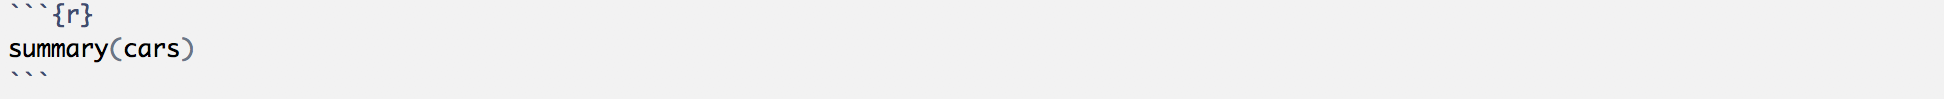
\includegraphics{picture1.png} This will print both the R code and
results on the output file.

\begin{Shaded}
\begin{Highlighting}[]
\KeywordTok{summary}\NormalTok{(cars)}
\end{Highlighting}
\end{Shaded}

\begin{verbatim}
##      speed           dist       
##  Min.   : 4.0   Min.   :  2.00  
##  1st Qu.:12.0   1st Qu.: 26.00  
##  Median :15.0   Median : 36.00  
##  Mean   :15.4   Mean   : 42.98  
##  3rd Qu.:19.0   3rd Qu.: 56.00  
##  Max.   :25.0   Max.   :120.00
\end{verbatim}

\hypertarget{chunk-options}{%
\section{Chunk Options}\label{chunk-options}}

Chunk output can be customized with knitr option, arguments set in the
\{\} of a chunk header.

\textbf{Example.} Render the the following four R code chunks, and
compaire their output files. Match the following answers with the R code
chunks below.

\begin{enumerate}
\def\labelenumi{\arabic{enumi}.}
\tightlist
\item
  Both the R code and result don't appear in the output document.\\
\item
  The R code appers in the output document, but not the results.\\
\item
  The results appers in the output document, but not the R code.
\end{enumerate}

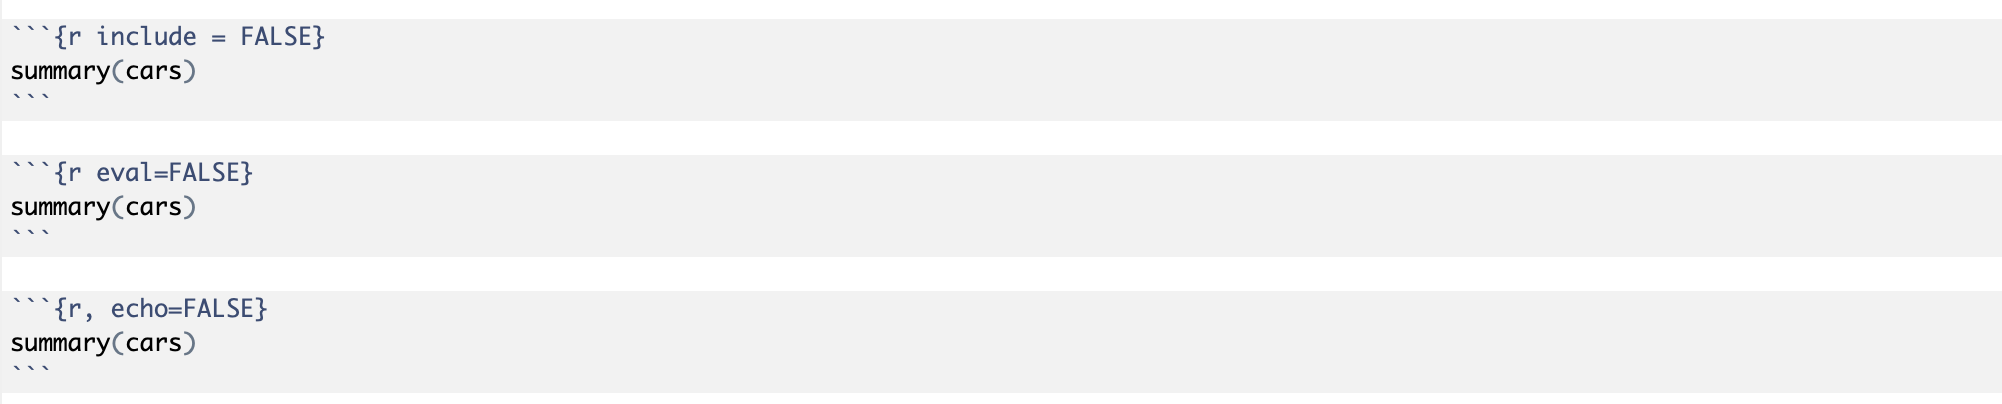
\includegraphics{picture2.png}

Here, I list seven arguments to customize the chunk output:

\begin{itemize}
\tightlist
\item
  \texttt{include\ =\ FALSE} prevents code and results from appearing in
  the output document. R Markdown still runs the code in the chunk, and
  the results can be used by other chunks.
\item
  \texttt{eval\ =\ FALSE} the source code appears in the output
  document, but not the results. R Markdown does NOT evaluate the code
  in the chunk.
\item
  \texttt{echo\ =\ FALSE} the source code does not appear in the output
  document, but the results appear. This is a useful way to embed
  figures.
\item
  \texttt{message\ =\ FALSE} prevents messages that are generated by
  code from appearing in the output document.
\item
  \texttt{warning\ =\ FALSE} prevents warnings that are generated by
  code from appearing in the output document.
\item
  \texttt{fig.cap\ =\ "..."} adds a caption to graphical results.
\item
  \texttt{fig.align\ =\ "..."} aligns the figure in the output document
  (left, right or center).
\end{itemize}

There are a large number of chunk options in knitr documented at
\url{https://yihui.name/knitr/options}.

\hypertarget{including-plots}{%
\section{Including Plots}\label{including-plots}}

We can embed plots, for example:

\begin{Shaded}
\begin{Highlighting}[]
\KeywordTok{hist}\NormalTok{(cars}\OperatorTok{$}\NormalTok{speed,}\DataTypeTok{breaks=}\DecValTok{10}\NormalTok{, }\DataTypeTok{xlab =}\StringTok{'Speed of Cars'}\NormalTok{, }\DataTypeTok{ylab=}\StringTok{'Number of Cars'}\NormalTok{, }\DataTypeTok{main=}\StringTok{''}\NormalTok{)}
\end{Highlighting}
\end{Shaded}

\includegraphics{Lab-RMarkdown_files/figure-latex/unnamed-chunk-2-1.pdf}

We can also custimize the figures, such as

\begin{figure}

{\centering \includegraphics[width=0.5\linewidth]{Lab-RMarkdown_files/figure-latex/unnamed-chunk-3-1} 

}

\caption{Histogram of speed of 50 cars recoreded in the 1920s.}\label{fig:unnamed-chunk-3}
\end{figure}

\textbf{Note.}

\begin{enumerate}
\def\labelenumi{\arabic{enumi}.}
\tightlist
\item
  To make this ordered list, I've an empty line after the last word
  \texttt{Note.}
\item
  The \texttt{echo\ =\ FALSE} parameter was added to the code chunk to
  prevent printing of the R code that generated the plot.\\
\item
  We use \texttt{fig.align=\textquotesingle{}center\textquotesingle{}}
  to allign the figure on the center of the output document.\\
\item
  The \texttt{fig.cap=\textquotesingle{}\ \textquotesingle{}} add a
  caption to the figure. The pdf document includes the figure number in
  front of the caption, such as \texttt{Figure\ 1.} however, the html or
  word outputs do not have this.
\end{enumerate}

\textbf{Example:} The following scatterplot may bew used to determine
relation between temperature in degrees Celsius and vapor pressure of
mercury in millimeters (of mercury).

\begin{Shaded}
\begin{Highlighting}[]
\KeywordTok{plot}\NormalTok{(pressure, }\DataTypeTok{col =} \StringTok{"blue"}\NormalTok{, }\DataTypeTok{pch=}\DecValTok{16}\NormalTok{)}
\end{Highlighting}
\end{Shaded}

\begin{center}\includegraphics[width=0.5\linewidth]{Lab-RMarkdown_files/figure-latex/unnamed-chunk-4-1} \end{center}

To see more tips and tricks for working with images and figures in R
Markdown documents, visit
\url{http://zevross.com/blog/2017/06/19/tips-and-tricks-for-working-with-images-and-figures-in-r-markdown-documents/}.

\hypertarget{two-figures-in-two-columns}{%
\section{Two figures in Two columns}\label{two-figures-in-two-columns}}

You can display two plots one beside each other. Add
\texttt{out.width=c(\textquotesingle{}50\%\textquotesingle{},\ \textquotesingle{}50\%\textquotesingle{}),\ fig.show=\textquotesingle{}hold\textquotesingle{}}
to your chunk header.

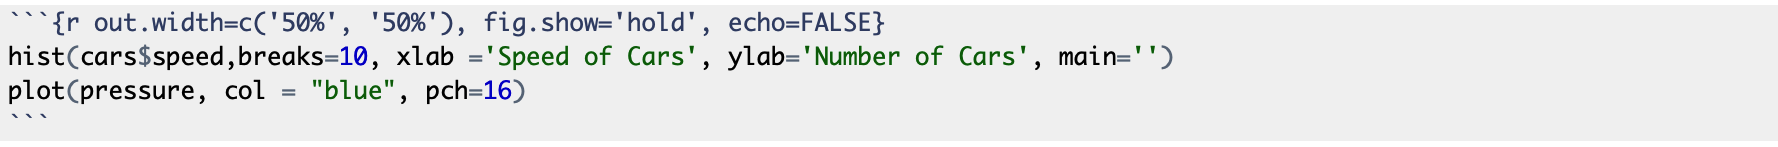
\includegraphics{picture5.png}

\includegraphics[width=0.5\linewidth]{Lab-RMarkdown_files/figure-latex/unnamed-chunk-5-1}
\includegraphics[width=0.5\linewidth]{Lab-RMarkdown_files/figure-latex/unnamed-chunk-5-2}

\hypertarget{tables}{%
\section{Tables}\label{tables}}

By default, R Markdown displays data frames and matrixes as they would
be in the R terminal (in a monospaced font). If you prefer that data be
displayed with additional formatting you can use the knitr::kable
function, as in the .Rmd file below.

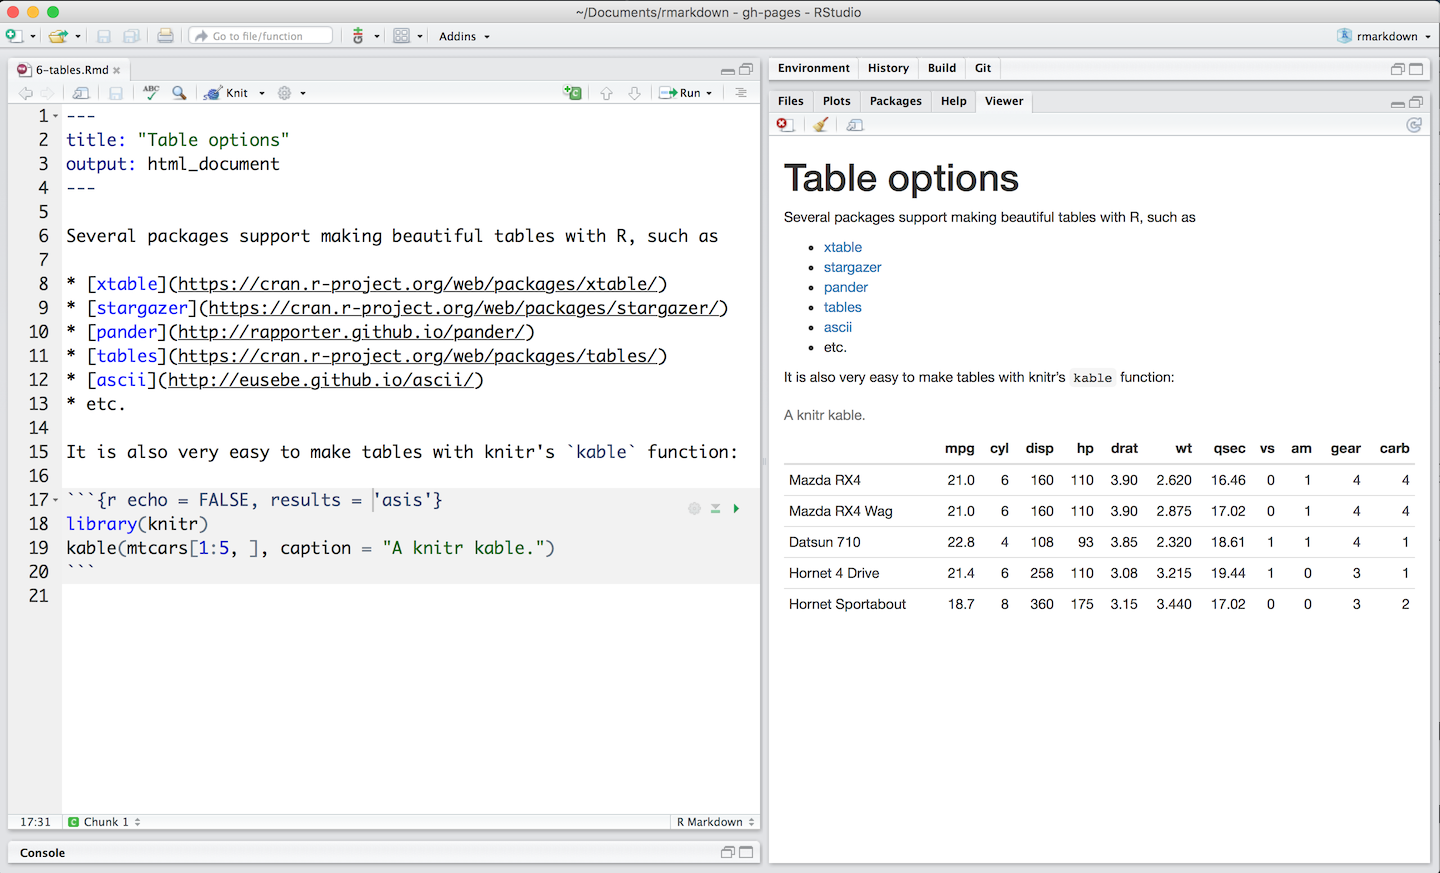
\includegraphics{tables-1-kable.png}

Note the use of the results=`asis' chunk option. This is required to
ensure that the raw table output isn't processed further by knitr.

\hypertarget{equations}{%
\section{Equations}\label{equations}}

Insert equation using Latex formating:

\begin{itemize}
\tightlist
\item
  for inline equation use write the equation between two dolar sign
  \texttt{\$\ equation\ \$}, for instance \(A = \pi*r^{2}\)
\item
  for centered equation use \texttt{\$\$\ equation\ \$\$}, for instance
  \[\int_0^{\pi^2/4} \sin\sqrt{x}\,dx\]
\end{itemize}

\hypertarget{comment-out-unused-text-in-r-markdown}{%
\section{Comment Out Unused Text in R
Markdown}\label{comment-out-unused-text-in-r-markdown}}

Extra yaml blocks can be used anywhere inside the document, and
commented out with \texttt{\#}


\includegraphics{picture6.png}

\hypertarget{text-formating}{%
\section{Text Formating}\label{text-formating}}

End a line with two spaces to start a new paragraph.

\emph{italics} and \emph{italics}

\textbf{bold} and \textbf{bold}\\
superscript\textsuperscript{2}

\sout{strikethrough}

\href{www.rstudio.com}{link}

\hypertarget{header-1}{%
\section{Header 1}\label{header-1}}

\hypertarget{header-2}{%
\subsection{Header 2}\label{header-2}}

\hypertarget{header-3}{%
\subsubsection{Header 3}\label{header-3}}

\hypertarget{header-4}{%
\paragraph{Header 4}\label{header-4}}

\hypertarget{header-5}{%
\subparagraph{Header 5}\label{header-5}}

Header 6

Add an horizontal line by adding 3 stars or 3 minus signs, e.i. *** or
---

Note that, the horizontal break needs to be surrounded by a beginning
and an ending new line.

\begin{center}\rule{0.5\linewidth}{\linethickness}\end{center}

\begin{center}\rule{0.5\linewidth}{\linethickness}\end{center}

\begin{quote}
block quote
\end{quote}

\begin{itemize}
\tightlist
\item
  unordered list
\item
  item 2

  \begin{itemize}
  \tightlist
  \item
    sub-item 1
  \item
    sub-item 2
  \end{itemize}
\item
  item 3
\end{itemize}

\begin{enumerate}
\def\labelenumi{\arabic{enumi}.}
\tightlist
\item
  ordered list
\item
  item 2

  \begin{itemize}
  \tightlist
  \item
    sub-item 1
  \item
    sub-item 2
  \end{itemize}
\item
  item 3
\end{enumerate}

\begin{longtable}[]{@{}ll@{}}
\toprule
Table Header & Second Header\tabularnewline
\midrule
\endhead
Table Cell & Cell 2\tabularnewline
Cell 3 & Cell 4\tabularnewline
\bottomrule
\end{longtable}

\hypertarget{global-options}{%
\section{Global Options}\label{global-options}}

To set global options that apply to every chunk in your file, call
\texttt{knitr::opts\_chunk\$set} in a code chunk. Knitr will treat each
option that you pass to \texttt{knitr::opts\_chunk\$set} as a global
default that can be overwritten in individual chunk headers.

\hypertarget{code-languages}{%
\section{Code Languages}\label{code-languages}}

The knitr can execute code in many languages besides R. Some of the
available language engines include:

\begin{itemize}
\tightlist
\item
  Python
\item
  SQL
\item
  Bash
\item
  Rcpp
\item
  Stan
\item
  JavaScript
\item
  CSS
\end{itemize}

To process a code chunk using an alternate language engine, replace the
\texttt{r} at the start of your chunk declaration with the name of the
language:

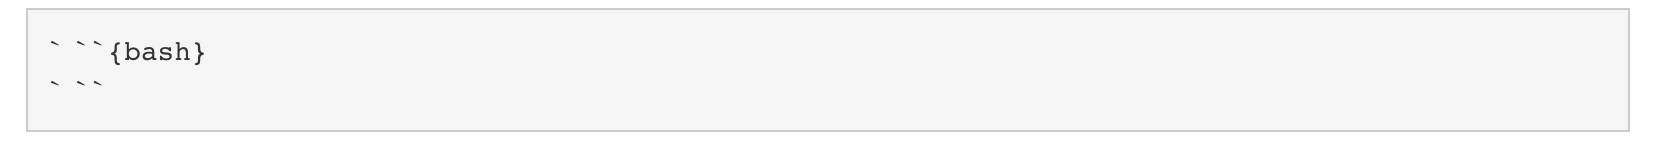
\includegraphics[width=0.9\textwidth,height=\textheight]{picture3.png}

Note that chunk options like \texttt{echo} and results are all valid
when using a language engine like python.


\end{document}
